A \textit{cold box} at CERN used in electronics tests for \dword{pdsp} is available for electronics testing in cold nitrogen gas. The cold box is designed to cycle one full-size \dword{apa} with the full set of \num{20} \dword{femb} through gaseous nitrogen temperatures around \SI{150}{K} to check out the \dword{apa} performance prior to installing the \dword{apa} into the \dword{pdsp} cryostat. It is designed to be a Faraday cage identical to the \dword{pdsp} cryostat and is read out by a complete \dword{ce} system for a single \dword{apa}, including a \dword{ce} flange and fully-loaded \dword{wiec} with five \dwords{wib} and one \dword{ptc}.

Preliminary results from the \dword{pdsp} cold box indicate that
the noise performance of the TPC readout will satisfy the DUNE \dword{fd} noise requirements of
\dword{enc}\,<\,\num{1000}\,e$^-$ on \dword{spmod}-length wires. These measurements suggest that the noise level in
\lar would be around \num{500}\,e$^-$ and \num{600}\,e$^-$ for the collection and induction plane channels,
respectively; this is well below the requirement.  The \dword{enc} and temperature of the second \dword{pdsp}
\dword{apa} delivered to CERN in the cold box are shown in Figure~\ref{fig:cb_results}.

\begin{dunefigure}
[\dword{enc} in electrons for several cases]
{fig:cb_results}
{\dword{enc} in electrons (left axis) for the wrapped induction wires (red and blue curves) and 
straight collection wires (green curve) as well as the temperature in degrees Kelvin (right axis) for the temperature
sensors in the CERN cold box (orange curves) as a function of cold cycle time in gaseous nitrogen for \dword{pdsp} \dword{apa}2. 
At the lowest temperature of \SI{160}{K}, the wrapped wires measured 480e$^-$ noise and the straight 
wires \num{400}\,e$^-$. This noise level is consistent with all other \dword{pdsp} \dwords{apa} tested in the cold box.}
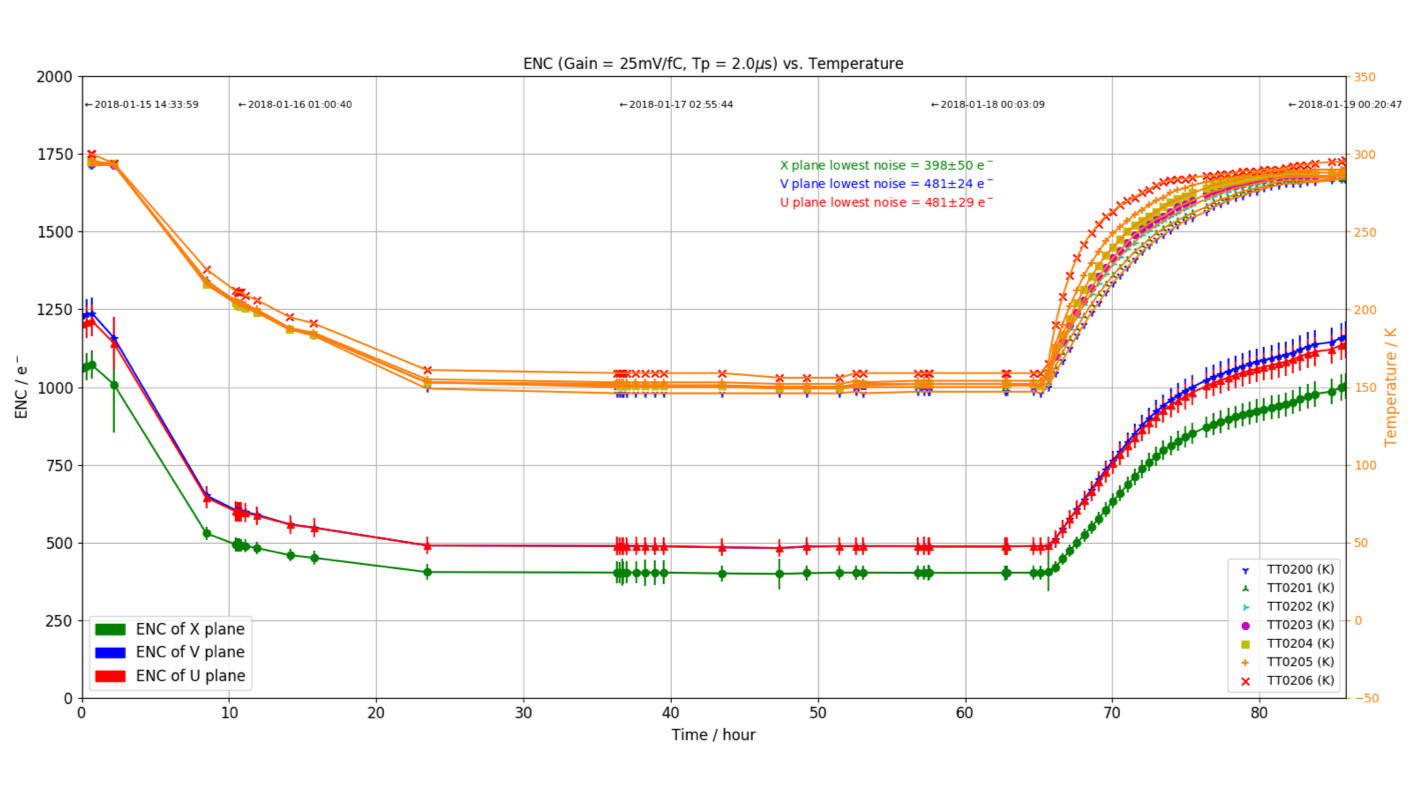
\includegraphics[width=0.73\linewidth]{tpcelec-apa2-results.png}
\end{dunefigure}
